\documentclass{sbthesis} % source: Dr. Keith Schubert
%\usepackage[pdftex]{graphicx}
\usepackage{graphicx}
\usepackage{verbatim}
\usepackage{textcomp}
\usepackage{setspace}
\usepackage{float}

%%%%%%%%%%%%%%%%%%%%%%%%%%%%%%%%%%%%%%%%%%%%%%%%%%%%%%%%%%%%%%%%%%%%%%
%
% NOTE: I didn't have to do this.  Maybe it's because I'm using Miktex.  -- David Turner
%
% Note: bibtex omits page number from first page of bibliography, 
% which is not acceptable under CSUSB rules.  The following
% command can be used to fix the problem.  For this to work,
% you need to insert \FixBib after the first line in the bbl file 
% that bibtex generates.  Do this each time the bibliography
% changes.
%
% Source: http://www.cs.ubc.ca/~murphyk/Teaching/latex_tips.txt
%
%%%%%%%%%%%%%%%%%%%%%%%%%%%%%%%%%%%%%%%%%%%%%%%%%%%%%%%%%%%%%%%%%%%%%%
\newcommand{\FixBib}{%    PUT \FixBib in file.bbl after first line
    \setlength{\parsep}{\parskip}%
    \setlength{\itemsep}{0cm}%
    \setlength{\topsep}{\parskip}%
    \setlength{\parskip}{0cm}%
    \setlength{\partopsep}{0cm}%
    \setlength{\listparindent}{\parindent}%
    \setlength{\labelwidth}{10pt}%
    \setlength{\labelsep}{0pt}%
    \setlength{\leftskip}{0pt}%
    \setlength{\leftmargin}{0pt}%
}


\title{My Master's Project Title}
\TitleLineTwo{A Template to Start From}
\author{David Turner}
\Department
\EmailAddress{dturner@csusb.edu}
\Advisor{George Georgiou}
\Committee{Kerstin Voigt}{Arturo I. Concepcion}
\CSUSBDate{March 2010}


\AbstractText{
This is an example Latex document that graduate students at CSUSB can use to format their master's project reports. The remainder of this abstract is irrelevant.  The term web application refers to a software system that provides a user interface through a web browser. Examples of web applications include blogs, wikis, online shopping, search engines, etc. Web application development became an important discipline following the adoption of the Internet by ordinary users. Many businesses now rely heavily on the web for both internal applications and to provide services to customers, and so there are many employment opportunities open to individuals with web development skills.

Web sites can be roughly classified as static or dynamic. Static web sites are those sites that use a web server to provide access to HTML documents that are stored in the file system. Dynamic web sites are those sites that construct the content of web pages from data that is stored in a database. The databases on which these dynamic sites are built are typically modified as a result of user interaction with site. Thus, users are presented with web pages that are uniquely generated for them based on their previous interactions with the site. The trend is for web pages to be generated from databases rather than being read from the file system.
}

\AcknowledgementText{
I would like to thank all the people with whom I have worked while pursuing my master's degree at California State University, San Bernardino (CSUSB). I wish I could list all their names but the list would be too long and I would still probably leave some people out. Studying in the School of Computer Science and Engineering at CSUSB has been a tremendous learning experience, both personally and professionally.

Thank you to the following faculty of the Computer Science and Engineering department for their invaluable guidance, advice, support, help, and patience during this project's long gestation: Dr. David Turner, Dr. Arturo Concepcion and Dr. Kerstin Voigt.

Special thanks to Rojer Wilco in the Department of Radio Devices. Without his valuable suggestions and support, the Internet wouldn't be a safe a place for online transactions as it is today.

I would also like to thank my wife for her undying support for my studies over the years. Finally, thanks to my parents who encouraged me all along. 
}

\begin{document}
\Project  % defined in sbthesis.cls 

\Chapter{Introduction}

The term web application refers to a software system that provides a user interface through a web browser. Examples of web applications include blogs, wikis, online shopping, search engines, etc.\cite{mysql-website} Web application development became an important discipline following the adoption of the Internet by ordinary users. Many businesses now rely heavily on the web for both internal applications and to provide services to customers, and so there are many employment opportunities open to individuals with web development skills.

Web sites can be roughly classified as static or dynamic. Static web sites are those sites that use a web server to provide access to HTML documents that are stored in the file system. Dynamic web sites are those sites that construct the content of web pages from data that is stored in a database. The databases on which these dynamic sites are built are typically modified as a result of user interaction with site. Thus, users are presented with web pages that are uniquely generated for them based on their previous interactions with the site. The trend is for web pages to be generated from databases rather than being read from the file system.

\section{Computer Languages Used for Web Application Development}

There are numerous languages and frameworks that are used for web application development. Java is one of the older and more established languages in which web applications have been developed. This book covers Java-based web application development using Servlets and JSP\cite{bauer2004}. This book also covers the news feed protocol RSS version 2.0, and REST-based web services.

Java is a strict object-oriented language in which all function calls are made to either static methods of classes or to non-static methods that are invoked through class instances. These classes are organized into namespaces called packages, so that unqualified class names do not need to be globally unique.

An application programming interface (API) is a specification that defines how user code can access system functionality. The Java API refers to the specification that defines how Java code may access functionality, such as opening a file in the file system, creating a socket connection with another process, creating a linked-list of objects, etc. For example, the following line creates an instance of the Socket class\cite{johnson2005}, which can be used to make TCP connections to other processes.

{\small
\begin{verbatim}
	  $ cd /opt
	  $ tar -zxvf apache-tomcat-VERSION.tar.gz
	  $ ln -s apache-tomcat-VERSION tomcat
\end{verbatim}
}

The above line of code can be simplified by importing the class java.net.Socket into the local namespace by adding the following line just after the package declaration of a java source code file.

import java.net.Socket;
The above import statement allows for the following simplified version of the socket creation code give above, in which the package prefix qualifiers are dropped from the Socket class.

{\small
\begin{verbatim}
Socket socket = new Socket("localhost", 8080);
\end{verbatim}
}

\section{The Servlet API}

The Socket class is an example of a class that is part of the core Java API, which is available in all standard Java virtual machine (JVM) environments. However, web applications typically additional functionality that is not part of the core Java API. In particular, conventional web applications need to be able to access functionality provided through the Servlet API. Implementations of the Servlet API are provided by third parties, such as Apache, IBM, Oracle, etc. In fact, the Servlet API is provided by something called a web container (or Servlet container), which is defined within an extensive specification called Java 2 Enterprise Edition (J2EE). A web container is actually a web server that loads and executes Java Servlets to process incoming requests from browsers (or other HTTP clients).

\section{Project Scope}

There's nothing like a good list to help organize the project scope.

\begin{itemize}
    \item I'm an item
    \item I'm also an item
    \item I'm the third and last item
\end{itemize}

\section{Definitions, Acronyms, and Abbreviations}

The definitions, acronyms, and abbreviations used in the document are described in this section.

\begin{itemize}
    \item API: Application Program Interface is a set of routines that an application uses to request and carry out low-level services performed by a computer's operating system; also, a set of calling conventions in programming that defines how a service is invoked through the application.
    \item CEL: The College of Extended Learning at California State University, San Bernardino.
    \item CELORS: The College of Extended Learning Online Registration System.
    \item CentOS: A freely available operating system that is based on Red Hat Enterprise Linux.
    \item CSUSB: California State University, San Bernardino.
    \item DHCP: Dynamic Host Configuration Protocol is a computer networking protocol used by devices (DHCP clients) which dynamically distributes the IP address to the destination host.
    \item DNS: The Domain Name System is a hierarchical naming system for computers, services, or any resource connected to the Internet or a private network.
    \item Hibernate\label{def:hibernate}: An object-relational mapping (ORM) library for the Java language which provides a framework for mapping an object-oriented domain model to a traditional relational database.
    \item HTML: HyperText Markup Language is the authoring language used to create documents on the World Wide Web.
    \item HTTPS: Hypertext Transfer Protocol Secure is a combination of the Hypertext Transfer Protocol and a network security protocol. This security protocol operates at a lower sublayer, encrypting an HTTP message prior to transmission and decrypting a message upon arrival.
    \item IEP: International Extension Programs is a unit of the College of Extended Learning.
    \item J2EE: Java 2 Platform Enterprise Edition is a platform-independent, Java-centric environment from Sun Microsystems, Inc., for developing, building, and deploying Web-based enterprise applications online. The J2EE platform consists of a set of services, APIs, and protocols that provide the functionality for developing multitiered, Web-based applications.
    \item Java: Java is a object-oriented, cross-platform programming language from Sun Microsystems.
    \item Java Servlet: Java Servlet technology provides Web developers with a simple, consistent mechanism for extending the functionality of a Web server and for accessing existing business systems.
    \item JDBC: Java Database Connectivity is an API for the Java programming language that defines how a client may access a database. It provides methods for querying and updating data in a database. JDBC is oriented towards relational databases.
    \item Join Table (also known as a ``Link Table" or ``Junction Table"): A Join Table is table that contains common fields from two tables. It is on the many side of a one-to-many relationship with the other table. It is employed when dealing with many-to-many relationships in a database.
    \item JSP: Java Servlet Page is a server-side technology. JSPs have dynamic scripting capabilities that work in tandem with HTML code, separating the page logic from the static elements to help make the HTML more functional (i.e., dynamic database queries).
    \item MVC\label{def:mvc}: Model-View-Controller is an architectural pattern used in software engineering to isolate business logic from user interface considerations.
    \item Osher: Osher Lifelong Learning Institute is a unit of the College of Extended Learning. 
    \item MySQL\label{mysql}: MySQL is a relational database management system which runs as a server providing multi-user access to a number of databases.
    \item Paypal\label{paypal}: Paypal is an e-commerce business allowing payments and money transfers to be made through the Internet. Paypal serves as an electronic alternative to traditional paper payment methods such as checks and money orders.
    \item PCI: Payment Card Industry.
    \item PCI DSS\label{def:PCI_DSS}: Payment Card Industry Data Security Standard. The standard was created to help organizations that process card payments to prevent credit card fraud through increased controls around data and its exposure to compromise. 
    \item Section 508: In 1998, the U.S. Congress amended the Rehabilitation Act to require Federal agencies to make their electronic and information technology accessible to people with disabilities. Section 508 was enacted to eliminate barriers in information technology, to make available new opportunities for people with disabilities, and to encourage development of technologies that will help achieve those goals.
    \item Session: A session is a collection of related clients which can exchange data via defined communication paths. The session maintains the state-associated communication paths and may interact with an object which encapsulates a defined session-management policy.
    \item Socket: An endpoint for communication between two machines.
    \item Spring Framework\label{def:spring}: (Spring, for short) is an open-source application framework for the Java platform.
    \item TCP/IP: Transmission Control Protocol on top of the Internet Protocol provides a reliable, point-to-point communication channel that client-server applications on the Internet use to communicate with each other. To communicate over TCP, a client program and a server program establish a connection to one another. Each program binds a socket to its end of the connection. To communicate, the client and the server each read from and write to a socket bound to the connection.
    \item Tomcat: Apache Tomcat is a servlet container. Tomcat implements the Java Servlet and the Java Server Pages (JSP) specifications and provides a ``pure Java" HTTP Web server environment for Java code to run.
    \item UML: The Unified Modeling Language is the industry-standard language for specifying, visualizing, constructing, and documenting the artifacts of software systems.
\end{itemize}

\Chapter{Database Design}

The CELORS implements an object/relational mapping (ORM) framework through Hibernate. Hibernate provides the bridge between the database, which is MySQL, and the Java application by storing application objects in the database, rather than writing and maintaining an abundance of code to store and retrieve objects. In short, object/relational mapping (ORM) is the automated persistence of objects to the tables in a relational database. Hibernate uses required metadata to describe the mapping between the objects and the database. Table~\ref{table:staff_metadata} is a mapping metadata for the staff table.

\vspace{3em}

\begin{table}[H]
\caption{Staff Table Metadata}\label{table:staff_metadata}
	\textbf{ }
\small
\begin{tabular}{p{13cm}}
\begin{verbatim}
<?xml version='1.0'?>
<!DOCTYPE hibernate-mapping PUBLIC 
         "-//Hibernate/Hibernate Mapping DTD 3.0//EN" 
         "http://hibernate.sourceforge.net/hibernate-mapping-3.0.dtd">
<hibernate-mapping>
  <class name="cel.bus.Staff" table="staff" lazy="true"> 
     <cache usage="read-write" />
     <id name="id" column="id" type="long">
        <generator class="increment"/>
     </id> 
     <property name="username" type="string" unique="true"/>
     <property name="passwordDigest" type="string" column="password" />
     <property name="firstName" type="string"/>
     <property name="lastName" type="string"/>
     <property name="email" type="string" />
     <property name="regNotify" type="boolean"/> 
     <property name="specialRegNotify" type="boolean" />
     <property name="manageCoursePermission" 
             column="manage_course_permission" type="boolean"/>
     <property name="processStudentPermission" 
             column="process_student_permission" type="boolean"/>
     <property name="manageReportPermission" 
             column="manage_report_permission" type="boolean"/>
  </class>
</hibernate-mapping>
\end{verbatim}
\end{tabular}
\end{table}

\section{Data Analysis}

To effectively store all necessary data, a database with 18 tables was reconstructed. Six of them are join tables (also called association tables) and five tables were dropped from the previous version because they were unused or CEL's business rules had changed. All tables used in the CELORS project store plain text data. The Entity Relational (ER) diagram for the CELORS system is shown in Figure~\ref{fig:er_diagram}.

\vspace{3em}

\begin{figure}[H]
\begin{center}
    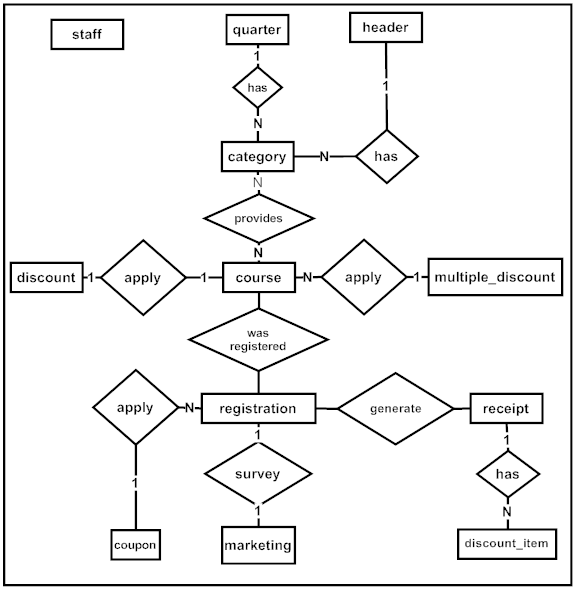
\includegraphics[height=5.3in]{images/ER_diagram.png}
    \caption{Entity Relational Diagram}
    \label{fig:er_diagram}
\end{center}
\end{figure}

\section{Database Specification}

The Key field indicates whether the column is indexed. A value of PRI indicates that the column is part of the table's primary key. UNI indicates that the column is part of a UNIQUE index. The MUL  value indicates that multiple occurrences of a given value are allowed within the column.

\subsection{Database Schema Logical Model - Relational Schema}

I'm a subsection.  This appears in the TOC.
\Chapter{Conclusion and Future Direction}

\section{Conclusion}

The College of Extended Learning Online Registration System facilitates the processing of registrations for the College of Extended Learning (CEL). Based upon the feedback received from CEL staff, and new regulation requirements from the CSU administration, this version of the system represents an improvement over the previous version in many aspects.

First, the course manager has more control of the CELORS. For instance, when the Osher membership fee or the maximum number of courses allowed to take per Osher quarter changes, the course manager has full control to change the number as desired and it is affected immediately. Currently, the course manager must contact CEL's contract programmer to modify source codes and which usually takes several hours to reveal. The clone function makes populating courses descriptions into a new quarter catalog a more expedient process.

Second, this version of the CELORS makes the payment process more accurate, efficient, and secure. In older verisons, CEL staff extract encrypted payment information from the system and stored into a portable device, usually a floppy disk or flash drive. They bring it to an isolated computer to decrypt and print registrations out. They then enter credit card information and fees one-by-one into the credit card machine. A typo could cause the payment to not go through or charge the wrong person. With automating the payment process through Paypal, CEL staff still has control of the payments but less chance for human errors. The registrations won't go through the CELORS if students make any mistakes during the payment process.

Finally, by using the newer technologies of Spring Framework and Hibernate provided, the system runs more efficiently and is easier to maintain and implement.

\section{Future Direction}

The development of the project progressed much more slowly than anticipated. The project itself has a great deal of life ahead of it though, which can be viewed as a positive aspect, especially if future programmers take interest enough to complete the remaining tasks.

A short list of work that could be done in the future are:
\begin{itemize}
    \item{Implementing marketing analysis reports functionalities}
    \item{Adding the Paypal refund functionality}
    \item{Adding a pay-through-Paypal-page function (redirect registrating students to the CEL-customized Paypal page)}
\end{itemize}


%\appendix  not used, from Dr. Schubert's template

\nocite{*}
\Bibliography{main}

\end{document}
